\documentclass[11pt]{article}
\usepackage{certmachine}

\title{A certified hot-spots family beyond the proven classes}
\author{\cmauthor}
\date{September 2026}

\begin{document}
\maketitle

\begin{abstract}
Rauch's hot spots conjecture asks whether a second Neumann eigenfunction
of the Laplacian attains its extrema only on the boundary. After fifty
years the proofs cover special classes---domains with symmetry, lip
domains, Euclidean triangles---while for convex quadrilaterals the
question is open and current work addresses symmetric subcases. We prove
the hot spots property for a single explicit domain outside every class
with an analytic proof: the convex trapezoid with vertices $(0,0)$,
$(1,0)$, $(17/20,9/10)$, $(1/4,9/10)$, which has no axis of symmetry and
is not a lip domain. The proof is computer-assisted and fully certified:
a deterministic chain of eight interval-arithmetic computations
(re-runnable in under two minutes) that (i) localizes the second
Neumann eigenvalue in $[12.020976127,\,12.022398359]$ and certifies its
simplicity through Crouzeix--Raviart lower bounds with interval inertia
counts; (ii) bounds the boundary defect of an exact 40-mode
Fourier--Bessel trial by $1.2369\cdot10^{-5}$ using interval Taylor jets,
giving $\norm{u-\phih}_{L^2}\le 6.5353\cdot10^{-5}$ for the true
eigenfunction $\phih$; and (iii) excludes interior extrema on a
three-part partition of the domain---a deep core by a solid-mean value
argument with interior witnesses, a boundary collar by a swept
centered-form evaluation with reflected pointwise bounds (zero residual
cells), and four corner tips by certified Fourier--Bessel corner
expansions, where the cold corner requires a Bessel ladder identity to
evaluate a singular second derivative whose divergence has the helpful
sign. We then extend the result from the point to an
interval: the same property is certified for \emph{every} $c$ in
$[0.845,0.85]$, where $C=(c,9/10)$, by seventeen chunks each carrying
the full six-stage chain --- to our knowledge the first certified
positive-measure family of hot-spots domains outside the proven classes.
Beyond the specific theorems, the paper documents a reusable
instrument set for certified Neumann eigenfunction analysis on polygons
and a ledger of failure modes of interval rigor that exact
falsifiers caught during construction.
\end{abstract}

\section{Introduction}

In 1974 J.~Rauch proposed what is now called the \emph{hot spots
conjecture} \cite{Rauch}: for a ``nice'' domain $\Omega\subset\R^2$, a
second Neumann eigenfunction of the Laplacian attains its maximum and
minimum on the boundary. The name records the physical picture: an
insulated plate with generic initial heat distribution develops its
hottest and coldest points on the edge, since the long-time temperature
profile is dominated by the second Neumann mode.

The subsequent fifty years produced a landscape of partial results whose
boundary is remarkably sharp. The conjecture is \emph{false} in general:
Burdzy and Werner constructed a planar counterexample with two holes
\cite{BurdzyWerner}, and Burdzy later one hole \cite{Burdzy2005};
Kleefeld located numerical counterexample candidates with striking
simplicity \cite{Kleefeld}; and de~Dios Pont showed failure even for
\emph{convex} domains once the dimension is high enough \cite{dDP}, with
quantitative refinements in \cite{dDPHT}. It is \emph{true} for domains
with two axes of symmetry (Jerison--Nadirashvili \cite{JerisonNadirashvili}),
for lip domains---domains between two Lipschitz graphs with constant
$\le 1$---(Atar--Burdzy \cite{AtarBurdzy}, following
Ba\~nuelos--Burdzy \cite{BanuelosBurdzy}), for classes of acute triangles
(Siudeja \cite{Siudeja}), and---in the landmark of the area---for all
Euclidean triangles (Judge--Mondal \cite{JudgeMondal}). For convex
planar domains the conjecture is expected to hold, and Steinerberger
proved the extrema live near the ``tips'' up to an inradius-scale
neighborhood \cite{Steinerberger}; but beyond triangles no unconditional
class is known. For convex \emph{quadrilaterals}---the immediate
frontier after \cite{JudgeMondal}---the problem is open; current work
treats symmetric subcases \cite{SymQuad}.

This paper proves the hot spots property for one explicit convex
quadrilateral chosen to sit outside every proven class.

\begin{theorem}\label{thm:main}
Let $\Omega$ be the trapezoid with vertices
\[
A=(0,0),\qquad B=(1,0),\qquad C=\Bigl(\tfrac{17}{20},\tfrac{9}{10}\Bigr),
\qquad D=\Bigl(\tfrac14,\tfrac{9}{10}\Bigr),
\]
and let $\varphi$ be a second Neumann eigenfunction of $-\Delta$ on
$\Omega$ (the second eigenvalue $\mu_1$ is simple---part of the
certificate---so $\varphi$ is unique up to scale). Then $\varphi$
attains its maximum and its minimum on $\partial\Omega$ only.
\end{theorem}

The domain is convex with side slopes $6$ and $18/5$; it has no axis of
symmetry (so \cite{JerisonNadirashvili,SymQuad} do not apply), both
slanted sides are steeper than slope $1$ (so it is not a lip domain in
any orientation and \cite{AtarBurdzy} does not apply), and it is not a
triangle. To our knowledge Theorem~\ref{thm:main} makes $\Omega$ the
first domain outside all analytically proven classes for which the hot
spots property is a theorem. The result is a single specimen, not a
class; its point is that the \emph{certified-computation} route to such
theorems now exists end to end, with the corner analysis---the part of
\cite{JudgeMondal} that consumed the most delicate analysis---carried
out by interval arithmetic against exact corner expansions.

\paragraph{Method in one paragraph.}
Floating-point computation proposes; interval arithmetic certifies. A
Crouzeix--Raviart eigenvalue computation with exact rational assembly
and interval inertia counts brackets the low Neumann spectrum and proves
$\mu_1$ simple (\S\ref{sec:spectrum}). A method-of-particular-solutions
trial $u$---a 40-term Fourier--Bessel sum over the four corners, an
\emph{exact} Helmholtz solution---is frozen, and its only defect, the
Neumann boundary flux, is certified small by interval Taylor-jet
quadrature (\S\ref{sec:trial}). A residual--gap argument in the spirit
of Moler--Payne turns the defect into $L^2$, $H^1$ and eigenvalue
enclosures for the true eigenpair (\S\ref{sec:eigenpair}). A solid-mean
lemma converts $L^2$ control of the error into pointwise control at
interior points, which powers a value argument: certified suprema over a
partition of the interior are beaten by certified values at two interior
witness points (\S\ref{sec:core}--\ref{sec:collar}). What survives is a
neighborhood of each corner, where $\varphi$ equals its Fourier--Bessel
corner expansion exactly; certified expansion coefficients kill three
corners outright, and the cold corner falls to a no-critical-point
argument plus a second-order Taylor bound off the Neumann edge whose
input is a singular second derivative evaluated through a Bessel ladder
identity (\S\ref{sec:tips}). Section~\ref{sec:assembly} assembles the
theorem; \S\ref{sec:lessons} records the methods ledger;
Appendix~\ref{app:repro} specifies the artifact and its trust base.

\paragraph{Relation to prior computational work.}
The trial-function technology descends from Fox--Henrici--Moler
\cite{FHM} and the eigenvector bounds of Moler--Payne \cite{MolerPayne},
revived and stabilized by Betcke--Trefethen \cite{BetckeTrefethen}; the
certified lower bounds use the framework of Liu \cite{Liu2015} in the
form quoted by You--Xie--Liu \cite{YouXieLiu} with the Crouzeix--Raviart
element \cite{CrouzeixRaviart}. The two literature constants entering
the certificate are Liu's framework theorem and the interpolation
constant $0.1893\,h_K$; everything else is computed and
interval-certified in the artifact. For the culture of computer-assisted
proof by validated numerics see \cite{vdBL,Tucker}; unlike
numerical-evidence studies of hot spots (e.g.\ \cite{Kleefeld}), every
inequality below is a proved bound about the exact eigenfunction.

\section{The specimen and the architecture of the proof}\label{sec:specimen}

Write $0=\mu_0<\mu_1\le\mu_2\le\cdots$ for the Neumann eigenvalues of
$-\Delta$ on $\Omega$. The corner data of the specimen are exact:

\begin{center}
\begin{tabular}{@{}lllll@{}}
\toprule
vertex & coordinates & opening $\omega$ & \quad(radians) & exponent $\nu=\pi/\omega$ \\
\midrule
$A$ & $(0,0)$        & $\arctan(18/5)$      & $1.299849$ & $2.41694$ \\
$B$ & $(1,0)$        & $\arctan 6$          & $1.405648$ & $2.23499$ \\
$C$ & $(17/20,9/10)$ & $\pi-\arctan 6$      & $1.735945$ & $1.80973$ \\
$D$ & $(1/4,9/10)$   & $\pi-\arctan(18/5)$  & $1.841744$ & $1.70587$ \\
\bottomrule
\end{tabular}
\end{center}

All four openings are strictly less than $\pi$ (convexity) and all
exponents lie in $(1,3)$: eigenfunctions are $C^0$ up to the corners,
with first derivatives blowing up like $r^{\nu-1}$ only for $\nu<1$
(never here) and second derivatives like $r^{\nu-2}$ at $C$ and $D$
(where $\nu<2$)---the analytic fact that shapes both the choice of trial
basis and the endgame at the cold corner.

The certified float landscape (a guide, not an input to any proof step):
the boundary maximum of the normalized eigenfunction sits \emph{at}
vertex $A$ with value ${\approx}\,2.151$ and the boundary minimum on the
top edge near $C$ at ${\approx}\,(0.8305, 0.9)$ with value
${\approx}\,{-2.000}$.

\paragraph{Normalization.}
The certificate chain produces a frozen trial $u$ with
$\norm{u-c_1\varphi_1}_{L^2}\le E$ for the $L^2$-normalized second
eigenfunction $\varphi_1$ and some scalar $c_1$. All arguments concern
$\phih:=c_1\varphi_1=u-e$; extrema locations are invariant under scaling,
and the sign is fixed by $\phih(A)>0$.

\paragraph{The partition.}
An interior extremum is excluded zone by zone (Figure~\ref{fig:zones}):
\begin{itemize}
\item \textbf{Core} --- depth $\ge 0.075$ from $\partial\Omega$: a
certified supremum over an adaptive cell cover is strictly beaten by a
certified value at an interior witness (\S\ref{sec:core}).
\item \textbf{Collar} --- depth $<0.075$ and distance $\ge 0.11$ from
every vertex: the same value argument, cell by cell, with pointwise
error bounds \emph{reflected} across the nearby Neumann edge
(\S\ref{sec:collar}).
\item \textbf{Four tips} --- distance $\le 0.11$ from a vertex: exact
corner expansions with certified coefficients (\S\ref{sec:tips}).
\end{itemize}
Completeness of the partition is elementary given convexity
(\S\ref{sec:assembly}).

\begin{figure}[t]
\centering
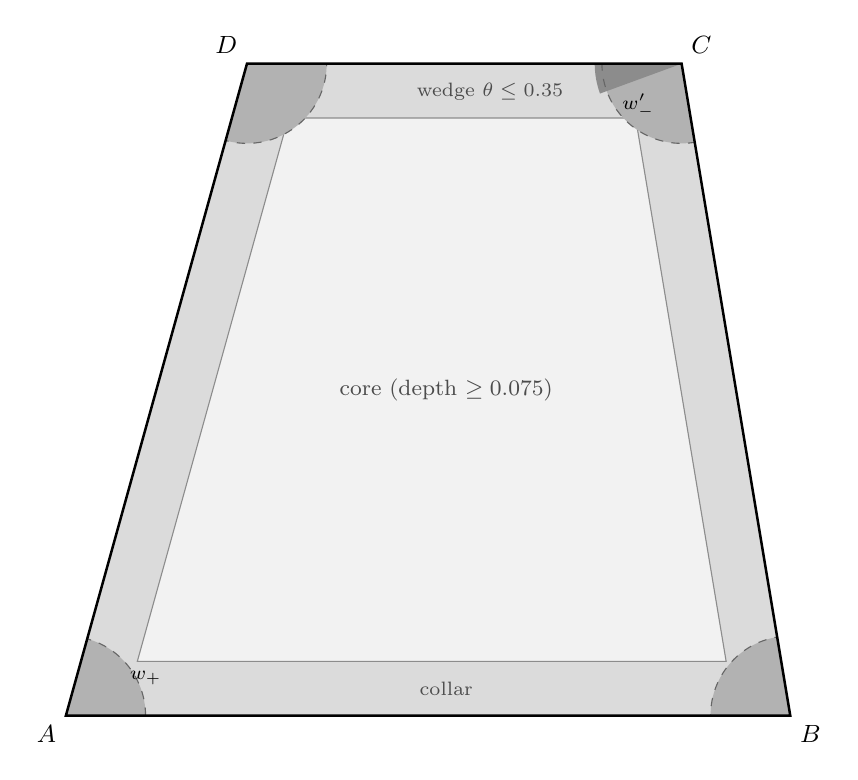
\begin{tikzpicture}[scale=9.2]
% collar ground
\path[fill=black!14] (0,0) -- (1,0) -- (0.85,0.9) -- (0.25,0.9) -- cycle;
% core
\path[fill=black!5] (0.09867,0.075) -- (0.91147,0.075) -- (0.78647,0.825) -- (0.30701,0.825) -- cycle;
\draw[black!45, line width=0.4pt] (0.09867,0.075) -- (0.91147,0.075) -- (0.78647,0.825) -- (0.30701,0.825) -- cycle;
% tips + wedge, clipped
\begin{scope}
\clip (0,0) -- (1,0) -- (0.85,0.9) -- (0.25,0.9) -- cycle;
\fill[black!30] (0,0) circle (0.11);
\fill[black!30] (1,0) circle (0.11);
\fill[black!30] (0.85,0.9) circle (0.11);
\fill[black!30] (0.25,0.9) circle (0.11);
\fill[black!45] (0.85,0.9) -- ++(180:0.12) arc (180:200.1:0.12) -- cycle;
\draw[black!60, dashed, line width=0.4pt] (0,0) circle (0.11);
\draw[black!60, dashed, line width=0.4pt] (1,0) circle (0.11);
\draw[black!60, dashed, line width=0.4pt] (0.85,0.9) circle (0.11);
\draw[black!60, dashed, line width=0.4pt] (0.25,0.9) circle (0.11);
\end{scope}
% boundary
\draw[line width=0.9pt] (0,0) -- (1,0) -- (0.85,0.9) -- (0.25,0.9) -- cycle;
% witnesses
\node at (0.0456,0.039) {\scriptsize$\blacklozenge$};
\node[anchor=west, font=\scriptsize] at (0.075,0.052) {$w_+$};
\node at (0.8305,0.881) {\scriptsize$\lozenge$};
\node[anchor=north east, font=\scriptsize] at (0.826,0.872) {$w_-'$};
% vertex labels
\node[anchor=north east, font=\small] at (0,0) {$A$};
\node[anchor=north west, font=\small] at (1,0) {$B$};
\node[anchor=south west, font=\small] at (0.85,0.9) {$C$};
\node[anchor=south east, font=\small] at (0.25,0.9) {$D$};
% zone labels
\node[font=\footnotesize, black!70] at (0.525,0.45) {core (depth $\ge 0.075$)};
\node[font=\scriptsize, black!70] at (0.525,0.0375) {collar};
\node[anchor=east, font=\scriptsize, black!70] at (0.70,0.862) {wedge $\theta\le 0.35$};
\end{tikzpicture}
\caption{The zone map. Core: value argument against the witness $w_+$
(max side) and $w_-'$ (min side), margins $5.4\cdot10^{-2}$ and
$1.2\cdot10^{-2}$. Collar: 2{,}166 cells, reflected bounds, zero
residual. Tips (radius $0.11$, dashed): exact corner expansions ---
$A$ dies radially, $B$ and $D$ by value, $C$ by a no-critical-point
sector plus the wedge, where $\phih_{nn}\ge 13.04$.}
\label{fig:zones}
\end{figure}

\section{Certified spectrum: bracketing and simplicity}\label{sec:spectrum}

\paragraph{Upper bounds.}
A conforming Galerkin basis (products of cosines and shifted Legendre
polynomials pulled back from the unit square, dimension $169$) is
assembled with \emph{exact rational} integrals---the only
non-polynomial integral family is expanded in a positive series with a
certified tail---so the stiffness and mass matrices are known as
rational intervals of width ${\sim}10^{-16}$. Interval Rayleigh--Ritz
(min--max over float-selected trial subspaces, evaluated in interval
arithmetic) gives certified
\begin{equation}\label{eq:uppers}
\mu_1 \le 12.04181916, \qquad \mu_2 \le 14.12684697 .
\end{equation}
A regression on the rectangle $1\times\frac{9}{10}$ reproduces
$\mu_1=\pi^2$ to all displayed digits.

\paragraph{Lower bounds.}
Nonconforming Crouzeix--Raviart \cite{CrouzeixRaviart} eigenvalues on a
mesh with exact rational vertices bound the continuous spectrum from
below through Liu's framework \cite{Liu2015}: if
$\norm{u-P_hu}_{L^2}\le C_h\,|u-P_hu|_{1,h}$ then
$\lambda_k \ge \lambda_{h,k}/(1+C_h^2\lambda_{h,k})$, with
$C_h=0.1893\,h_{\max}$ from the per-triangle interpolation bound
$\norm{u-\Pi_hu}_{0,K}\le 0.1893\,h_K\,|u-\Pi_hu|_{1,K}$
\cite{YouXieLiu}. (In the Neumann configuration both spaces are taken
mean-zero; the projection differs from $\Pi_h$ by a constant, which only
shrinks the $L^2$ norm.) The \emph{discrete} eigenvalues are bounded by
interval \emph{inertia} counts: a diagonally pivoted right-looking
interval elimination of $K-\sigma M$ combined with float symmetric
scaling (both congruences, so Sylvester's law applies) counts
eigenvalues below the exact rational shift $\sigma$. The result, on a
456-dof mesh:
\begin{equation}\label{eq:spec}
\mu_1 \in [11.892663,\ 12.04181916], \qquad \mu_2 \ge 13.955936,
\end{equation}
and \emph{exactly one} nonzero eigenvalue lies below $13.955936$:

\begin{proposition}[simplicity]\label{prop:simple}
$\mu_1$ is a simple eigenvalue, and $\mu_2-\mu_1 \ge 1.914$.
\end{proposition}

This gap is the load-bearing input: it makes ``the'' second
eigenfunction well defined and powers the eigenpair enclosure below.

\section{The trial and its certified boundary defect}\label{sec:trial}

\paragraph{Why not Galerkin.}
A float diagnostic closed the naive route before rigor was built on it:
for the smooth Galerkin basis the \emph{strong} residual
$\norm{-\Delta\tilde u-\lambda\tilde u}_{L^2}$ \emph{diverges} with
basis size ($6.3\to9.7$ for $N=8\to20$), driven by the corner
singularities ($r^{\nu-2}$, $\nu\in(1.71,2.42)$). Eigenvalue min--max
is unaffected, but the eigenfunction certificate had to move to a basis
with the corners built in.

\paragraph{The trial.}
The method of particular solutions \cite{FHM,BetckeTrefethen} with four
corner Fourier--Bessel fans: at each vertex, modes
$J_{k\nu}(\sqrt{\lam}\,r)\cos(k\nu\theta)$, $k=0,\dots,9$, in local
polar coordinates ($\theta$ measured from one adjacent edge, $\nu$ the
corner exponent). Each mode solves $-\Delta u=\lam u$ \emph{exactly}
and has exact Neumann data on its two adjacent edges; the only defect
of any linear combination is the Neumann flux on the far edges. The
float scan (Betcke--Trefethen subspace angles, stabilized by
rank-truncated SVD, column normalization, and an absolute noise floor;
see \S\ref{sec:lessons}) is deterministic and selects
\[
\lam = 12.021687243,
\]
inside the certified bracket \eqref{eq:spec}, with float defect
$9.0\cdot10^{-6}$, stable from $K{=}10$ through $K{=}18$ per corner.
The $40$ coefficients at $K{=}10$ are frozen as exact doubles; from
this point nothing about $u$ is tuned.

\paragraph{Certified defect.}
On each edge, the flux of each far fan is a composition of
$J_\nu,J_\nu'$ and trigonometric factors of the local angle. Writing
$s(\tau)=s_0+\tau$ for arclength relative to a far corner (with
constant transverse offset $d$, $r^2=s^2+d^2$, $\theta'=+d/r^2$), the
flux $f(\tau)$ closes under differentiation via the Bessel ODE, so
\emph{order-2 interval Taylor jets} $(f,f',f'')$ are computed without
any hand-derived third-order chain rule. A certified cell rule
\[
\textstyle\int_{\text{cell}} f^2
\;\le\; h f(m)^2 + \tfrac{h^3}{12}f'(m)^2
+ 2R\bigl(h|f(m)|+\tfrac{h^2}{4}|f'(m)|\bigr) + R^2 h,
\qquad R=\tfrac{h^2}{8}\,\mathrm{mag}\,f''(\text{cell}),
\]
summed over $700$ cells per edge gives
\begin{equation}\label{eq:defect}
\norm{\dnu u}_{L^2(\partial\Omega)} \le D = 1.2369\cdot10^{-5},
\qquad \sup_{\text{edge}}|\dnu u| \le 1.4\cdot10^{-5}\ \text{per edge},
\end{equation}
$37\%$ above the float value---the interval overhead is benign. Every
jet order used is validated against an independent float evaluation
(``bridges''), a guard installed after a sign bug in $\theta'$ inflated
the certified defect $1000\times$ \emph{while all value bridges passed}
(\S\ref{sec:lessons}, item 5).

\section{The eigenpair certificate}\label{sec:eigenpair}

Green's identity turns the boundary defect into a weak residual: for
$v\in H^1(\Omega)$,
$\int_\Omega \nabla u\cdot\nabla v - \lam u v = \int_{\partial\Omega}(\dnu u)\,v$,
so with the certified trace constant (star-shaped form, rational center
$x_0=(21/40,\,9/20)$)
$\norm{v}_{L^2(\partial\Omega)}\le C_{\mathrm{tr}}\norm{v}_{H^1}$,
$C_{\mathrm{tr}}=2.6427$, the expansion coefficients $c_k$ of
$u=\sum c_k\varphi_k$ obey
\begin{equation}\label{eq:parseval}
\sum_k c_k^2\,\frac{(\mu_k-\lam)^2}{1+\mu_k} \;\le\; \varepsilon^2,
\qquad \varepsilon = C_{\mathrm{tr}}\,D = 3.2687\cdot10^{-5}.
\end{equation}
Combining \eqref{eq:parseval} with the spectrum localization
\eqref{eq:spec} (exactly one nonzero eigenvalue below $13.955936$) and
the certified norm bound $\norm{u}_{L^2}\ge c_1 \ge 0.166$ yields, with
$F=\max\bigl(\lam^{-2},\,(1+\mu_2^{\mathrm{lo}})/(\mu_2^{\mathrm{lo}}-\lam)^2\bigr)=3.9975$
and $G=\mu_2^{\mathrm{lo}}(1+\mu_2^{\mathrm{lo}})/(\mu_2^{\mathrm{lo}}-\lam)^2=55.79$:

\begin{proposition}[eigenpair enclosure]\label{prop:eigenpair}
\begin{align}
\mu_1 &\in [12.020976127,\ 12.022398359]
&&\text{(width $1.42\cdot10^{-3}$, a $105\times$ tightening of CR)},
\notag\\
\norm{u-\phih}_{L^2} &\le E = 6.5353\cdot10^{-5}
= \sqrt{F}\,\varepsilon,
&&\text{(relative $3.9\cdot10^{-4}$)},
\notag\\
|u-\phih|_{H^1} &\le \varepsilon\sqrt{G} = 2.4415\cdot10^{-4}.
\notag
\end{align}
\end{proposition}

This is a self-contained residual--gap argument of Moler--Payne type
\cite{MolerPayne}; the certified CR localization replaces the a priori
spectral information assumed there.

\section{Pointwise bounds and the core zone}\label{sec:core}

$L^2$ control of $e=u-\phih$ becomes pointwise control through an
explicit solid-mean identity, chosen over boundary-integral
representations because it needs no Bessel-$Y$ machinery: for
$-\Delta w=f$ on $B_R(x_0)\subset\Omega$,
\[
w(x_0)=\frac{1}{|B_R|}\int_{B_R} w+\int_{B_R}G_R f,\qquad
G_R(r)=\frac{1}{2\pi}\Bigl(\ln\frac{R}{r}-\frac{R^2-r^2}{2R^2}\Bigr),\qquad
\norm{G_R}_{L^2(B_R)}=R\sqrt{\frac{I_0}{2\pi}},
\]
with $I_0=\int_0^1\bigl(-\ln t-\tfrac{1-t^2}{2}\bigr)^2 t\,dt =
\frac{5}{48}$ \emph{exactly} (derived by hand, reverified numerically in
the artifact). Applied to $e$, which satisfies
$-\Delta e=\mu_1e+(\lam-\mu_1)u$ with $|\lam-\mu_1|\le 7.12\cdot10^{-4}$:
\begin{equation}\label{eq:solidmean}
|e(x_0)| \;\le\; \frac{E}{\sqrt{\pi}\,R}
+ R\sqrt{\tfrac{I_0}{2\pi}}\Bigl(\mu_1^{\mathrm{up}}E
+ |\lam-\mu_1|\,\norm{u}_{L^2}\Bigr),
\qquad B_R(x_0)\subset\Omega .
\end{equation}
At depth $0.075$ this certifies $|e|\le 5.5\cdot10^{-4}$; at the witness
depths below, ${\sim}10^{-3}$.

\paragraph{The value argument.}
No boundary values are ever needed. Two interior witnesses are placed
just inside the boundary extrema: $w_+$ at depth $0.033$ near $A$, and
$w_-'$ at depth $0.019$ under the boundary minimum. Certified through
\eqref{eq:solidmean}:
\[
\phih(w_+)\ \ge\ 2.126029, \qquad -\phih(w_-')\ \ge\ 1.993811 .
\]
An adaptive branch-and-bound cover of the core (1{,}473 cells, centered
form: cell value $\le$ center value $+$ magnitude of cell gradient
$\times$ half-diagonal) certifies
\[
\sup_{\mathrm{core}}\phih \le 2.071924, \qquad
\sup_{\mathrm{core}}(-\phih) \le 1.960684 .
\]

\begin{lemma}[core zone]\label{lem:core}
$\phih$ has no interior extremum at depth $\ge 0.075$: an interior
maximum would satisfy
$\phih(x^*)\ge\phih(w_+)\ge 2.126029>2.071924$, a contradiction
(margin $5.4\cdot10^{-2}$); symmetrically for the minimum
(margin $1.2\cdot10^{-2}$).
\end{lemma}

\section{The collar}\label{sec:collar}

Cells at depth $<0.075$ sit too close to $\partial\Omega$ for
\eqref{eq:solidmean}. The fix is reflection: across an open Neumann
edge, the even reflection of $\phih$ extends it as an $H^1$ solution of
the same eigenvalue equation, so solid-mean balls may cross the edge.
The trial $u$ is \emph{not} exactly Neumann, so its reflection carries a
single-layer correction with density $2\dnu u$; its contribution to
\eqref{eq:solidmean} is bounded by
$\sup|\dnu u|\cdot 3R/\pi$ using the certified per-edge sup in
\eqref{eq:defect}---three orders below the budgets in play.

The sweep covers all 2{,}166 collar cells (depth $<0.075$, distance
$\ge0.11$ from every vertex) with the centered-form supremum plus
reflected error bounds, on both sides ($\pm\phih$), with two refinement
levels:

\begin{lemma}[collar]\label{lem:collar}
Every collar cell has certified
$\sup_{\mathrm{cell}}\phih < 2.126029$ and
$\sup_{\mathrm{cell}}(-\phih) < 1.993811$: \emph{zero residual cells}.
No interior extremum lies in the collar.
\end{lemma}

(The raw interval evaluation of the 40-term trial over a cell suffers
catastrophic cancellation---widths ${\sim}1$ at cell size $0.01$; the
centered form is what makes the sweep possible. See
\S\ref{sec:lessons}, item 4.)

\section{The corner tips}\label{sec:tips}

In the sector of opening $\omega$ at each vertex, Neumann separation
plus $H^1$ regularity (which excludes the singular Bessel-$Y$ family)
gives the \emph{exact} representation
\begin{equation}\label{eq:cornerexp}
\phih \;=\; \sum_{k\ge0} b_k\,J_{k\nu}(\sqrt{\mu_1}\,r)\cos(k\nu\theta),
\qquad \nu=\pi/\omega,
\end{equation}
convergent in the closed sector. The coefficients $b_0,b_1,b_2$ are
certified by $L^2$ extraction over an annulus $r\in[0.03,0.09]$:
angular orthogonality makes the own-fan contribution of $u$ exact, the
far-fan part is integrated by second-order midpoint cells, and the
contamination by $e$ is controlled by $E$; a Parseval argument bounds
the tail $\sum_{k\ge3}$. Values, gradients and second derivatives of
\eqref{eq:cornerexp} are then interval-evaluated on each tip
($r\le0.11$) with certified geometric tails. Float guides:
$b_0\approx 2.151,\ 0.854,\ -2.000,\ -1.558$ at $A,B,C,D$---every tip
has $|b_0|\ge0.85$, so values separate cleanly from both extremal
levels wherever the extremum is not adjacent.

\begin{lemma}[tips $A$, $B$, $D$]\label{lem:tipsABD}
On $r\le0.11$:
\begin{itemize}
\item[$B$:] $\phih\in[0.7566,\ 0.8965]$ --- both sides dead by value.
\item[$D$:] $\phih\in[-1.6643,\ -1.3515]$ --- both sides dead by value.
\item[$A$:] $\phih\in[2.0153,\ 2.2195]$ --- min side dead by value; and
$\partial_r\phih<0$ throughout the sector (certified bound
$\le-0.0499$; an inner disk factorization gives $\le-10.0$ near the
vertex). An interior maximum at an interior point of the tip would be
an interior critical point of $\phih$; there is none. Hence no interior
extremum in tip $A$.
\end{itemize}
\end{lemma}

\paragraph{The cold corner $C$.}
The max side is dead by value ($\phih\le-1.8465$ on the tip). The min
side is the delicate one: the boundary minimum lies on the top edge at
distance ${\approx}0.02$ from the tip boundary, and the radial
$b_0/b_1$ cancellation locus passes through the sector. The tip splits
into two pieces, with $\theta$ measured from the top edge $CD$:

\emph{(i) The sector $\theta\in[0.35,\omega]$.} The squared gradient of
\eqref{eq:cornerexp} is minorized by a quadratic form in
$c=\cos(\nu\theta)$ (the ``min-form''), interval-minimized in closed
form over $c\in[-1,1]$; this certifies $|\nabla\phih|>0$ on
$r\in[10^{-5},0.11]$, and an analytic leading-order argument covers
$r<10^{-5}$. No critical point, hence no interior extremum, in this
piece.

\emph{(ii) The wedge $\theta\in[0,0.35]$, $r\le0.12$.} Here the
argument is transverse monotonicity from the Neumann edge. For a point
at (signed) distance $n$ from the top edge with foot $a$:
\[
\phih(a,n)\;=\;\phih(a,0)+\tfrac{n^2}{2}\,\phih_{nn}(a,\xi)
\qquad\text{(no first-order term: Neumann)},
\]
so a certified $\inf\phih_{nn}>0$ over the wedge forces
$\phih(\text{interior point})>\phih(\text{foot})\ge\min_{\partial\Omega}\phih$
--- no interior wedge point can attain the minimum.

The input $\phih_{nn}=-\mu_1\phih-\phih_{tt}$ requires the tangential
second derivative of \eqref{eq:cornerexp}, whose terms diverge like
$r^{\nu-2}$ ($\nu=1.80973$) with cancelling signs---exactly what
interval arithmetic cannot see through: a naive polar-split Hessian
returns widths that swallow the answer. The resolution is an identity
that performs the cancellation analytically. Differentiating a
Helmholtz corner mode twice along the fixed direction $\theta=0$ and
using the $J$ recurrences:
\begin{equation}\label{eq:ladder}
\partial_t^2\Bigl[J_{\nu}(\sqrt{\mu}\,r)\cos(\nu\theta)\Bigr]
=\frac{\mu}{4}\Bigl[
J_{\nu+2}(\sqrt{\mu}\,r)\cos\bigl((\nu{+}2)\theta\bigr)
+J_{\nu-2}(\sqrt{\mu}\,r)\cos\bigl((\nu{-}2)\theta\bigr)
-2J_{\nu}(\sqrt{\mu}\,r)\cos(\nu\theta)\Bigr],
\end{equation}
one interval evaluation per mode, no subtraction of near-equal singular
quantities---note the \emph{negative} fractional order $\nu-2\approx
-0.19$, which the special-function layer supports with closed-form
falsifiers. The geometry cooperates: the singular $k{=}1$ term has
$b_1<0$, so $\phih_{tt}\to-\infty$ and hence $\phih_{nn}\to+\infty$ as
$r\to0$---the corner singularity works \emph{for} the bound.

\begin{lemma}[tip $C$]\label{lem:tipC}
On the tip at $C$: the maximum side is dead by value; on the wedge,
$\phih_{nn}\ge13.04$ (outer piece; inner piece $\ge11.65$), and no
interior point of the sector piece is critical. No interior extremum
lies in tip $C$.
\end{lemma}

\section{Assembly}\label{sec:assembly}

\begin{proof}[Proof of Theorem~\ref{thm:main}]
\emph{Partition completeness:} every interior point has depth
$\ge0.075$ (core), or depth $<0.075$ and distance $\ge0.11$ from all
vertices (collar), or distance $<0.11$ from some vertex; in the last
case convexity places it inside that vertex's sector, and the tip
arguments run on the full sector $r\le0.11$ (the wedge to $0.12$).

\emph{Maximum.} Suppose $x^*\in\Omega$ (interior) attains
$\max_{\overline\Omega}\phih$. Then
$\phih(x^*)\ge\phih(w_+)\ge2.126029$. But $x^*$ lies in the core
($\sup\le2.071924$, Lemma~\ref{lem:core}: contradiction), or a swept
collar cell (certified $\sup<2.126029$, Lemma~\ref{lem:collar}:
contradiction), or tip $B$, $C$ or $D$ (values $\le0.8965$, $\le-1.8465$
--- on the relevant side --- and $\le-1.3515$, Lemmas~\ref{lem:tipsABD}
and \ref{lem:tipC}: contradiction), or tip $A$ --- where an interior
maximum forces $\nabla\phih(x^*)=0$, contradicting
$\partial_r\phih<0$ (Lemma~\ref{lem:tipsABD}).

\emph{Minimum.} Symmetric, with $w_-'$: core
($1.960684<1.993811$), swept collar cells, tips $A$, $B$, $D$ by value,
and tip $C$ by the no-critical-point sector plus the monotone wedge
(Lemma~\ref{lem:tipC}).

Hence both extrema of $\phih$ --- equivalently of any second Neumann
eigenfunction, by simplicity (Proposition~\ref{prop:simple}) and scale
invariance --- are attained on $\partial\Omega$ only.
\end{proof}

\section{From a point to an interval: the band}\label{sec:band}

A single certified domain invites the reply that it is a lucky specimen.
This section removes that reply.

\begin{theorem}[the band]\label{thm:band}
For every $c\in[0.845,\,0.85]$ let $\Omega_c$ be the trapezoid with
vertices $A=(0,0)$, $B=(1,0)$, $C=(c,9/10)$, $D=(1/4,9/10)$. Then
$\mu_1(c)$ is simple and the second Neumann eigenfunction of $-\Delta$
on $\Omega_c$ attains its maximum and its minimum on $\partial\Omega_c$
only.
\end{theorem}

The interval is tiled by seventeen closed chunks --- sixteen of width
$3\cdot10^{-4}$ from $0.85$ down to $0.8452$, plus $[0.845,0.8452]$ of
width $2\cdot10^{-4}$ --- each carrying the full six-stage chain of
Sections~\ref{sec:spectrum}--\ref{sec:tips}. Adjacent chunks are closed
and share endpoints, so their union is the closed interval with no gap.
The specimen of Section~\ref{sec:specimen} is $c=17/20=0.85$ and is
covered independently at the right endpoint.

\paragraph{Parametrisation.} Per chunk $[c_{\mathrm{lo}},c_{\mathrm{hi}}]$
put $c=c_{\mathrm{hi}}+\sigma H$ with $\sigma\in[-1,0]$ and
$H=c_{\mathrm{hi}}-c_{\mathrm{lo}}$. The trial family
$u(x,\sigma)=\sum_i a_i(\sigma)\psi_i(x)$ has \emph{fixed},
$c$-independent modes $\psi_i$ anchored at the $c_{\mathrm{hi}}$ frames,
with degree-three polynomial coefficients $a_i(\sigma)$; so $u$ is an
exact cubic in $\sigma$ at every point and $-\Delta u=\tilde\lambda
(\sigma)u$ holds exactly for every $\sigma$. Two facts made this work
where a naive $c$-sweep does not. Raw multiple-precision-shooting
coefficients are wild between nearby $c$ --- they vary by seven orders
--- so the family is solved once, point-normalised, rather than
per-$c$. And frozen frames carry a branch cut along the frame ray, so
the anchor is placed at the chunk's \emph{right} end, keeping every cut
ray outside every $\Omega_c$ in the chunk.

\paragraph{Certified values, worst over all seventeen chunks.}
\begin{center}
\begin{tabular}{ll}
\toprule
uniform spectrum & $\mu_1(c)\ge 11.85157$, $\mu_2(c)\ge 13.90774$ \\
boundary defect & $D_{\sup}\le 8.11\cdot10^{-5}$ \\
eigenvalue window & $\mu_1(c)\in[12.01166,\,12.04931]$ \\
eigenpair error & $\norm{u_\sigma-c_1\varphi_{1,c}}_{L^2}\le
4.39\cdot10^{-4}$ \\
zone margins & $\ge +2.47\cdot10^{-4}$ (max side),
$\ge +6.41\cdot10^{-4}$ (min side) \\
collar survivors outside corner windows & $0$, every cell, every chunk \\
corner witnesses & $\hat\varphi(w_+)\ge 0.98692$,
$-\hat\varphi(w_-')\ge 0.92692$ \\
tip $C$ & $b_1\le -0.8791<0$ certified on every chunk \\
\bottomrule
\end{tabular}
\end{center}
The uniform spectral pair gives simplicity for every $c$, and every
eigenvalue window lies strictly inside $(11.85157,\,13.90774)$, so
simplicity is never in question. The whole band cost about thirteen
hours single-core, roughly forty-five minutes per chunk, with the defect
stage dominating.

\paragraph{A resolution model, and its test.} The binding resource is
the number of $\sigma$-cells: the per-cell defect scales with cell width,
so a coarse cell rides a multiple of the median defect and the zone stage
fails first at a chunk's left end. Chunk $[0.8491,0.8494]$ did exactly
that, at worst margin $-1.1\cdot10^{-6}$. The model predicted that
raising the cell count from $12$ to $18$ would buy about
$+4\cdot10^{-3}$ of margin and sixteen or more chunks of runway. It then
delivered: all fifteen remaining chunks certified on the first attempt,
with zone margins between $+3.4\cdot10^{-3}$ and $+1.4\cdot10^{-2}$. We
report this because a resolution model that predicts correctly is more
reusable than the fix it recommended --- and note that the two thinnest
margins on the whole band belong to the two chunks built at the old
resolution, not to any chunk the model governed.

\paragraph{What the band does not claim.} It is an interval in
\emph{one} parameter of a four-parameter moduli space of convex
quadrilaterals. It is not the quadrilateral conjecture, and it is not a
census. The fence list of Section~\ref{sec:open} applies unchanged.

\section{Methods and lessons}\label{sec:lessons}

The chain was built in one session against a standing test discipline:
every certified computation ships with \emph{exact falsifiers} ---
closed-form cases that must be contained, and independent float
``bridges'' for every quantity certified. Six failure modes were caught
this way; we record them because each is generic to interval rigor,
not specific to this problem.

\begin{enumerate}
\item \textbf{Intervals enter last.} In a rational-core pipeline,
converting large intermediate quantities ($10^{13}$-sized Legendre
monomial coefficients) to intervals \emph{before} summation destroys
exact cancellation: one Gram entry acquired width $3.94$ (valid, but
useless). Summing in exact rationals and converting once gives width
$10^{-16}$.
\item \textbf{Pivot interval factorizations.} Unpivoted interval
$LDL^{\mathsf T}$ dies on a near-zero elimination pivot (an ordering
artifact, row 211 of 456). Diagonal-pivoted right-looking elimination
plus float symmetric scaling --- both congruences, so inertia is
preserved --- is robust.
\item \textbf{Measure the float convergence curve before building rigor
machinery.} The Galerkin strong residual diverges at the corners; a
week of interval code on that route would have certified nothing. One
diagnostic script killed it in advance and forced the MPS architecture.
\item \textbf{Centered forms, not raw cell intervals.} The raw interval
value of a 40-term trial over a cell suffers multi-term cancellation
blowup (widths ${\sim}1$); the centered form (point value $+$ cell
gradient $\times$ half-diagonal) is what makes certified sup-covers
feasible. Similarly, MPS needs rank-truncated SVD, column
normalization, and an \emph{absolute} noise floor --- $J_\nu$ at large
$\nu$ is float noise, and normalizing noise manufactures fake angles.
\item \textbf{Bridge every derivative order used.} A sign error in
$\theta'$ left every \emph{value} bridge passing (values came from the
angle formula) while every $\tau$-derivative used the wrong angular
motion: term cancellation failed only in $f'$ and the certified defect
inflated $1000\times$. Value tests do not test jets.
\item \textbf{Clamp at domain guards.} Outward rounding pushes
square-sums to $-5\cdot10^{-324}$ and $\Gamma$'s argument below its
domain edge by one ulp; clamping (which only tightens) and extending by
the functional equation are part of the rigor model.
\end{enumerate}

\section{Open problems}\label{sec:open}

\begin{enumerate}
\item \emph{The census.} Every instrument above is parameterized by the
quadrilateral. The natural next step is a certified \emph{census} over
the moduli space of convex quadrilaterals --- interval shape boxes,
each box certified by the same chain with uniform constants --- toward
the statement that \emph{convex quadrilaterals have no hot spots}. The
obstructions are quantitative (near-degenerate gaps as symmetry is
approached, where $\mu_1$ ceases to be simple) rather than structural.
\item \emph{Sharper $\mu_1$.} The enclosure width $1.4\cdot10^{-3}$ is
defect-limited; larger fans and finer jet quadrature should reach
$10^{-8}$ at proportionate cost if the eigenvalue itself becomes the
object of interest.
\item \emph{Other specimens.} Domains further from every proven class
--- non-trapezoidal, near-degenerate, or with $\nu$ close to $1$ at a
cold corner --- test which parts of the chain are generic. The cold-%
corner wedge argument used here needs only $b_1\ne0$ with the helpful
sign; a specimen where it fails would need a genuinely new endgame.
\end{enumerate}


% AI-assistance disclosure per your policy — goes here before deposit.]

\appendix

\section{Reproducibility and trust base}\label{app:repro}

The artifact is a directory of deterministic Node.js scripts (no
dependencies beyond the bundled MIT-licensed interval/rational kernel);
each prints an explicit \texttt{ok}/\texttt{FAIL} line per check and a
final ALL-PASS verdict. The full chain reruns in ${\approx}100$ seconds
single-core (measured on the build machine, 2026-09-01, all scripts
ALL PASS):

\begin{center}
\small
\begin{tabular}{@{}lllr@{}}
\toprule
script & role & certified output & secs \\
\midrule
\texttt{test-ivspecial.js} & special-function layer & 47 exact falsifiers & 0.1 \\
\texttt{run-p2a.js}        & Galerkin uppers & $\mu_1\le12.04181916$, $\mu_2\le14.12684697$ & 7.1 \\
\texttt{run-p2a2.js}       & CR lowers + inertia & \eqref{eq:spec}, simplicity & 3.5 \\
\texttt{run-p2b-mps.js}    & float MPS trial (deterministic) & $\lam$, frozen coefficients & 15.2 \\
\texttt{cert-defect.js}    & interval Taylor-jet flux & \eqref{eq:defect} & 4.6 \\
\texttt{cert-assemble.js}  & eigenpair enclosure & Proposition~\ref{prop:eigenpair} & 4.4 \\
\texttt{cert-pointwise.js} & solid-mean + core sweep & Lemma~\ref{lem:core} & 6.8 \\
\texttt{cert-collar.js}    & reflected collar sweep & Lemma~\ref{lem:collar} & 7.3 \\
\texttt{cert-corner.js}    & corner expansions + tips & Lemmas~\ref{lem:tipsABD}, \ref{lem:tipC} & 49.9 \\
\bottomrule
\end{tabular}
\end{center}

\paragraph{Rigor model.}
Intervals are outward-rounded IEEE-754 doubles; exact quantities are
BigInt rationals, converted to intervals as the \emph{last} step of any
derivation. The special-function layer (interval $\Gamma$ by Spouge's
formula with defensively widened error term; $J_\nu$, $J_\nu'$ by power
series with certified alternating tails, including negative fractional
order) is tested against closed forms: $\Gamma$ at integers and
half-integers and its functional equation at fractional arguments;
$J_{1/2}$, $J_{3/2}$ closed forms; the three-term recurrence at the
specimen's actual $\nu$ values; derivative identities against central
differences.

\paragraph{Literature inputs.}
Exactly two: Liu's framework theorem and the Crouzeix--Raviart
interpolation constant $0.1893\,h_K$, both as stated in
\cite{YouXieLiu} (read against the source, not from memory).

\paragraph{Classical facts used.}
Neumann separation of variables in a sector together with $H^1$
regularity (excluding the $Y_\nu$ family) for \eqref{eq:cornerexp};
Green's identity on $\Omega$; the spectral theorem; Courant's nodal
bound. All are textbook-level and enter as stated hypotheses, not as
computations.

\paragraph{Float landscape.}
All float numbers quoted (boundary extremum locations and values,
coefficient guides) are labeled guides; no proof step consumes them.

\begin{thebibliography}{99}\small

\bibitem{Rauch} J.~Rauch, Five problems: an introduction to the
qualitative theory of partial differential equations, in:
\emph{Partial Differential Equations and Related Topics} (Tulane
Univ., 1974), Lecture Notes in Math.\ 446, Springer, 1975, pp.~355--369.

\bibitem{BanuelosBurdzy} R.~Ba\~nuelos, K.~Burdzy, On the ``hot
spots'' conjecture of J.~Rauch, \emph{J.\ Funct.\ Anal.} 164 (1999)
1--33.

\bibitem{BurdzyWerner} K.~Burdzy, W.~Werner, A counterexample to the
``hot spots'' conjecture, \emph{Ann.\ of Math.} 149 (1999) 309--317;
arXiv:math/9803030.

\bibitem{Burdzy2005} K.~Burdzy, The hot spots problem in planar
domains with one hole, \emph{Duke Math.\ J.} 129 (2005) 481--502.

\bibitem{JerisonNadirashvili} D.~Jerison, N.~Nadirashvili, The ``hot
spots'' conjecture for domains with two axes of symmetry, \emph{J.\
Amer.\ Math.\ Soc.} 13 (2000) 741--772.

\bibitem{AtarBurdzy} R.~Atar, K.~Burdzy, On Neumann eigenfunctions in
lip domains, \emph{J.\ Amer.\ Math.\ Soc.} 17 (2004) 243--265.

\bibitem{Siudeja} B.~Siudeja, Hot spots conjecture for a class of
acute triangles, \emph{Math.\ Z.} 280 (2015) 783--806.

\bibitem{JudgeMondal} C.~Judge, S.~Mondal, Euclidean triangles have no
hot spots, \emph{Ann.\ of Math.} 191 (2020) 167--211; Erratum,
\emph{Ann.\ of Math.} 195 (2022) 337--362; arXiv:2108.10386.

\bibitem{Steinerberger} S.~Steinerberger, Hot spots in convex domains
are in the tips (up to an inradius), \emph{Comm.\ Partial Differential
Equations} 45 (2020) 641--654.

\bibitem{Kleefeld} A.~Kleefeld, The hot spots conjecture can be false:
some numerical examples, \emph{Adv.\ Comput.\ Math.} 47 (2021) 85;
arXiv:2101.01210.

\bibitem{dDP} J.~de~Dios~Pont, The hot spots conjecture can fail for
convex domains in high dimensions, arXiv:2412.06344 (2024).


\bibitem{dDPHT} J.~de~Dios~Pont, S.~Hsu, Taylor
[initials to be completed], arXiv:2508.16321 (2025).

% the quantitative follow-up in high dimension.]

\bibitem{SymQuad} Hot spots for symmetric convex quadrilaterals,
arXiv:2604.19003 (2026).

% the state of the quadrilateral case as of 2026-09-01.]

\bibitem{Liu2015} X.~Liu, A framework of verified eigenvalue bounds
for self-adjoint differential operators, \emph{Appl.\ Math.\ Comput.}
267 (2015) 341--355.

\bibitem{YouXieLiu} C.~You, H.~Xie, X.~Liu, Guaranteed eigenvalue
bounds for the Steklov eigenvalue problem, \emph{SIAM J.\ Numer.\
Anal.} 57 (2019) 1395--1414; arXiv:1808.08148.

\bibitem{CrouzeixRaviart} M.~Crouzeix, P.-A.~Raviart, Conforming and
nonconforming finite element methods for solving the stationary Stokes
equations~I, \emph{RAIRO} 7 (1973) 33--75.

\bibitem{FHM} L.~Fox, P.~Henrici, C.~Moler, Approximations and bounds
for eigenvalues of elliptic operators, \emph{SIAM J.\ Numer.\ Anal.} 4
(1967) 89--102.

\bibitem{MolerPayne} C.~B.~Moler, L.~E.~Payne, Bounds for eigenvalues
and eigenvectors of symmetric operators, \emph{SIAM J.\ Numer.\ Anal.}
5 (1968) 64--70.

\bibitem{BetckeTrefethen} T.~Betcke, L.~N.~Trefethen, Reviving the
method of particular solutions, \emph{SIAM Rev.} 47 (2005) 469--491.

\bibitem{vdBL} J.~B.~van den Berg, J.-P.~Lessard, Rigorous numerics in
dynamics, \emph{Notices Amer.\ Math.\ Soc.} 62 (2015) 1057--1061.

\bibitem{Tucker} W.~Tucker, A rigorous ODE solver and Smale's 14th
problem, \emph{Found.\ Comput.\ Math.} 2 (2002) 53--117.

\end{thebibliography}


\section{An independent audit of the covering}\label{sec:covering-audit}

An interval theorem is a union of chunk theorems, and such a union fails on
\emph{covering} far more readily than on arithmetic. Two covering claims carry
the result and neither is visible inside any single certificate: the chunks
must tile the parameter interval with shared endpoints, and inside each chunk
the $\sigma$-cells must tile $[-1,0]$ in every stage that reports per-cell
numbers. A gap of $10^{-12}$ in either makes the interval statement false.

Both ladders were therefore re-derived from the stage records by a checker
sharing no code with the program that produced them. It confirms that the
17 chunks tile $[0.845, 0.85]$ and that
the 738 $\sigma$-cells tile $[-1,0]$ in each of the zones,
defect and eigenpair stages, and it re-derives every band-wide constant from
per-cell data rather than reading a summary: $\mu_1 \ge 11.85157$,
$\mu_2 \ge 13.90774$, thinnest zone margins
$2.470e-4$ and $6.410e-4$,
zero collar survivors outside the corner windows, and $\sup b_1 = -0.8791 < 0$
at corner $C$ on every chunk. Corner $C$ is identified by position rather than
by the sign of $b_1$, since corner $B$ also carries a negative $b_1$ and a
sign-based scan could not detect $C$ losing the property it is meant to verify.

\begin{remark}
The audit found 51 of the $\sigma$-cells to be
\emph{zero-width}, emitted where the refinement toward $\sigma = 0$ bottoms out
and duplicates a shared endpoint. Such a cell certifies an empty set, so it
cannot affect the covering, and the remaining cells still tile $[-1,0]$ in every
chunk and every stage. It is recorded rather than discarded because a
certificate covering nothing is worth counting, and because the same rule that
excludes these cells is what prevents a zero-width piece from papering over a
genuine hole.
\end{remark}

\end{document}
